\documentclass[../Cours.tex]{subfiles}
\usepackage{multicol}
\usepackage[thicklines]{cancel}

\begin{document}

\setcounter{chapitre}{31}
\chapitre{Soustraction de nombres relatifs}

\partie{Entre deux nombres}

\propriete{Soustraire un nombre revient à ajouter son opposé.}
\begin{listedexemples}
    \item[*] $(-4) - (-7) = (-4) \textcolor{rouge}{+} (\textcolor{rouge}{+}7)$
    \item[*] $(-9) - (+4) = (-9) \textcolor{rouge}{+} (\textcolor{rouge}{-}4)$
\end{listedexemples}

\remarque{Il est possible de simplifier l'écriture d'une addition de la façon suivante :%
\begin{itemize}[label=*]
    \item $(-5)+(-3) = -5-3$
    \item $(+7)+(-2) = 7-2$
\end{itemize}
}

\partie{Somme algébrique}

\methode{Lorsqu'il y a plusieurs additions et soustractions qui se succèdent dans un même calcul : %
\begin{itemize}[label=$\longrightarrow$]
    \item je transforme toutes les soustractions en additions
    \item je regroupe les termes positifs entre eux, et les termes négatifs entre eux
    \item je termine le calcul de gauche à droite
\end{itemize}}

\exemple{\begin{align*}
    &~~~~(-6) + (+3) - (-7) - (+4) + (+6) - (+2)\\
    &= (-6) + (+3) + (+7) + (-4) + (+6) + (-2)\\
    &= (+3) + (+6) + (+7) + (-6) + (-4) + (-2)\\
    &= (+16) + (-12)\\
    &= (+4)
\end{align*}
}

\partie{Distance algébrique}

\definition{La distance entre deux nombres est la différence entre le plus grand et le plus petit des deux.}


\clearpage
\begin{questions}
    \exercice ~~\textsc{Les nombres croisés}\\
    \begin{wrapfigure}{r}{0.4\linewidth}
    \begin{tikzpicture}
        \draw (0,0) grid (4,4);
        \draw[fill=noir] (0,0) rectangle (1,1) (1,1) rectangle (2,2) (2,0) rectangle (3,1) (3,2) rectangle (4,3) (2,3) rectangle (3,4);
    \end{tikzpicture}
    \end{wrapfigure}
    \textbf{Horizontalement :}
    \begin{enumerate}
        \item Opposé de 8 $\blacksquare$ Positif et négatif à la fois
        \item $-13+215-7-6$
        \item Opposé de $-5$ $\blacksquare$ $-(-6-6)$
        \item $-0.5+1.5$ $\blacksquare$ Opposé de l'opposé de $-6$
    \end{enumerate}
    \textbf{Verticalement :}
    \begin{enumerate}
        \item Entier relatif compris entre $-15,6$ et $-14,9$
        \item $(-3+7) - (4-88)$ $\blacksquare$ $(-4) - (-5)$
        \item $52+34 - (35-41) - (8-7)$
        \item $(-3) - (-3)$ $\blacksquare$ 2 dizaines et 6 unités
    \end{enumerate}
    
    \exercice \textsc{Échelles de température}\\
    
    Dans la vie de tous les jours, la température est mesurées en degrés Celcius (°C). Mais il existe une autre échelle de température, l'échelle Kelvin, définie de la manière suivante :
    
    \[ T_{Kelvin} = T_{°Celcius} + \num{273,15} \]
    
    Par exemple, \qty{30}{°C} = \qty{300.15}{K}.
    
        \question Convertir \qty{50}{°C}, \qty{-15}{°C} et \qty{23,67}{°C} en Kelvins
        \question Convertir \qty{350}{K}, \qty{5000}{K} et \qty{25}{K} en degrés Celcius
        \question À quelle température l'eau liquide devient solide ? À quelle température l'eau liquide bouille-t-elle ? Donner les réponses en degrés Celcius et en Kelvins.
        \question Le zéro absolu est la température la plus basse possible dans l'univers, elle correspond à \qty{0}{K}. Donner sa valeur en degrés Celcius.
        
    \exercice ~~\textsc{Carré magique}\\
    
    \begin{wrapfigure}{r}{0.4\linewidth}
    \vspace{-1cm}
    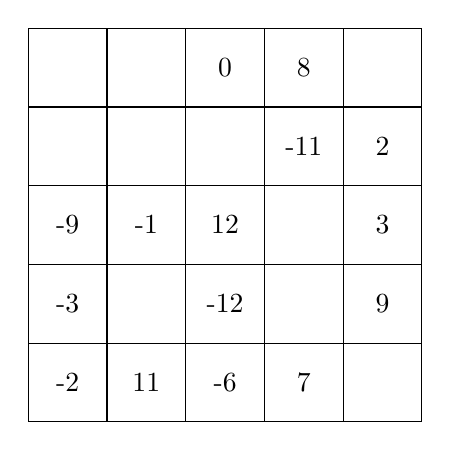
\begin{tikzpicture}
        \draw (1,1) grid (6,6);
        \node at (1.5,1.5) {-2};
        \node at (2.5,1.5) {11};
        \node at (3.5,1.5) {-6};
        \node at (4.5,1.5) {7};
        \node at (1.5,2.5) {-3};
        \node at (3.5,2.5) {-12};
        \node at (5.5,2.5) {9};
        \node at (1.5,3.5) {-9};
        \node at (2.5,3.5) {-1};
        \node at (3.5,3.5) {12};
        \node at (5.5,3.5) {3};
        \node at (4.5,4.5) {-11};
        \node at (5.5,4.5) {2};
        \node at (3.5,5.5) {0};
        \node at (4.5,5.5) {8};
    \end{tikzpicture}
    \end{wrapfigure}
    
    Si on additionne toutes les valeurs d'une ligne, d'une colonne ou d'une diagonale, on obtient 0. Tous les nombres entiers de $-12$ à $12$ sont présents dans le carré.\\
    Complète le carré magique ci-dessous.
    
    \vspace{2cm}
    \exercice ~~\textsc{Histoire antique}
    
    \question Compléter le tableau en remettant dans l'ordre croissant les dates suivantes : \\-356 ; -51 ; -1300 ; -330 ; -218 ; -776
    \question Compléter ensuite la colonne << durée >> en calculant la durée séparant chacun des évènements de l'Histoire antique.
    \begin{center}
    \begin{tabular}{|c|c|c|}\hline
    Évènements & année & durée \\\hline
    Naissance de Ramsès II  & & \\\hline
    $1^{er}$ jeux olympiques antiques  & & \\\hline
    Naissance d'Alexandre le grand & & \\\hline
    Naissance d'Euclide d'Alexandrie & & \\\hline
    Hannibal traverse les Alpes & & \\\hline
    Cléopâtre reine d'Égypte & & \\\hline
    \end{tabular}
    \end{center}
    
\end{questions}


\end{document}